\chapter{Redes Neurais Artificiais} \label{cap:redes}

Comparado com os computadores mais avançados que existem hoje, o cérebro humano ainda se mostra muito mais poderoso e eficaz do que as máquinas. O cérebro é capaz de processar informação a uma velocidade muito maior do qualquer computador convencional e realiza com facilidade tarefas como o reconhecimento de padrões e classificação de objetos, enquanto algoritmos tradicionais falham. 

Redes neurais artificiais foram criadas com inspiração no funcionamento e na estrutura do cérebro, como uma alternativa poderosa para resolver problemas que as arquiteturas tradicionais não eram capazes de resolver eficientemente. Essas redes emulam a estrutura cerebral natural, se utilizando de elementos distintos de processamento (neurônios) que se comunicam para realizar a tarefa desejada. 

Simon Haykin\cite{Haykin} define uma rede neural como "...um processador distribuído massivamente paralelo composto por unidades simples de processamento, que possui uma propensidade natural a armazenar conhecimento experimental e torná-lo disponível para uso."

As redes neurais artificiais são utilizadas para resolver problemas como ajuste de funções, classificação de objetos e reconhecimento de padrões. Este capítulo é uma continuação do Capítulo \ref{cap:fundament} e nele serão explicados conceitos importantes para o entendimento das redes artificiais, começando pelo seu elemento mais básico, o neurônio.

\section{Neurônios}

O neurônio é a estrutura básica do sistema nervoso central. É uma célula composta principalmente de três partes distintas: o corpo celular, os dendritos e o axônio. O corpo celular é a estrutra central do célula aonde está contido o núcleo do neurônio e são executados as suas funções vitais. Os dendritos são prolongamentos do corpo celular responsáveis por receber sinais e o axônio é uma extensão maior do corpo celular, responsável por enviar sinais a outros neurônios. Dois neurônios interagem em apenas  pontos de contato chamados sinapses. Nessas sinapses o axônio de um neurônio envia sinais para os dendritos de um segundo neurônio\cite{Kosabov}. A Figura \ref{fig:neuronio} ilustra a estrutura básica dos neurônios.

\begin{figure}
\centering
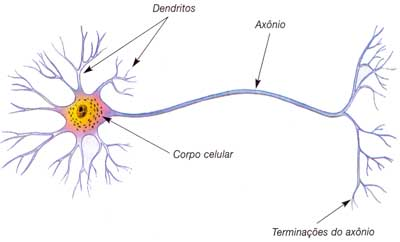
\includegraphics[width=.6\textwidth]{neuronio}
\caption{A estrutura básica de um neurônio humano. Extraída de \cite{neuronio}.}
\label{fig:neuronio}
\centering
\end{figure}

O neurônio artificial também possui três estruturas básicas semelhantes àquelas do neurônio natural. Seus três elementos básicos são: as entradas(análogas aos dendritos), a sáida(análoga ao axônio) e um núcleo de processamento. 

O neurônio pode ter uma ou mais conexões de entrada caracterizadas por um peso $wi$ e que recebe um valor $xi$. No núcleo do neurônio artificial há um somador que calcula o valor $u$ agregado das entradas, ponderadas pelo peso correspondente. O resultado dessa soma ponderada é então deslocado de um valor escalar e em seguida submetido a uma função chamada de função de ativação, que determina a saída final do neurônio. Em suma podemos descrever a saída de um neurônio $n$ que possui $i$ entradas através das seguintes equações:

\begin{equation}
 u_n = \sum_{j=1}^i x_jw_j
\end{equation}

\begin{equation}
s(n) = f(u_n + b)
\end{equation}

Aonde $u_n$ é o valor agregado das entradas, $x_j$ é a j-ésima entrada e $w_j$ o peso da conexão associada, $s(n)$ é a saída do neurônio, $f$ é a função de ativação e $b$ o deslocamento, ou $bias$ do neurônio $n$. A Figura \ref{fig:neuroartificial} ilustra a estrutura básica de um neurônio artificial.

\begin{figure}
\centering
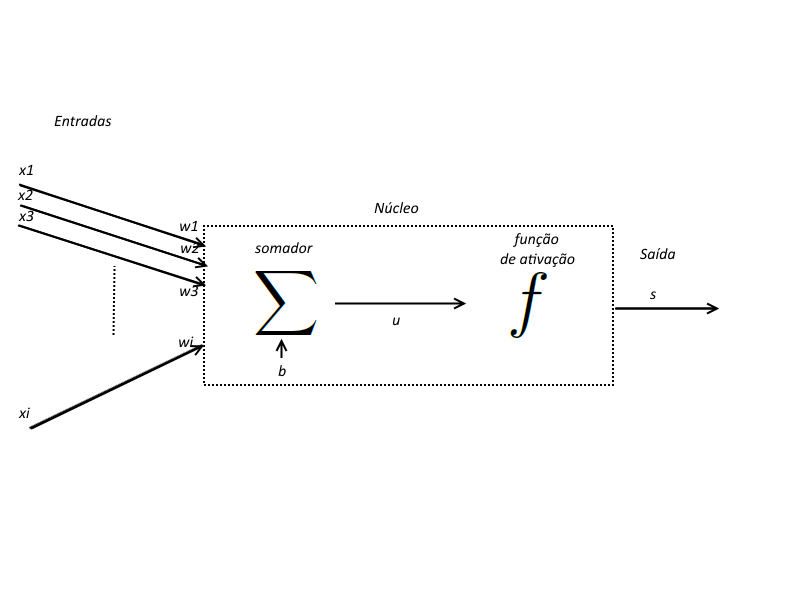
\includegraphics[width=.8\textwidth]{NeuronioArtificial}
\caption{A estrutura básica de um neurônio artificial.}
\label{fig:neuroartificial}
\centering
\end{figure}

Claramente, a função de ativação do neurônio é o grande fator que define o seu comportamento e consequentemente sua funcionalidade. Existem dois tipos básicos de funções de ativação\cite{Haykin}: a função degrau e a função sigmóide.

O neurônio mais simples possível tem sua saída regida por uma função degrau e saída binária. Isto é, se o valor agregado $u$ de suas entradas for maior que um determinado limiar, a sua saída será 1 e a saída será 0 caso contrário. Apesar de ser capaz de resolver alguns problemas, esse tipo de neurônio tem algumas desvantagens. Por vezes, alterações sutis podem representar a diferença entre os dois valores possíveis da sáida. Além disso, um alcance limitado de valores na saída prejudica o treinamento.

A escolha mais comum de de função de ativação para a construção de redes neurais é a família de funções sigmóides. Essas funções, que tem um gráfico com formato de \textit{S}, assumem valores contínuos entre 0 e 1, o que faz com que alterações sutis na entrada representem alterações mais sutis na saída, aumentando a qualidade da informação gerada pelo neurônio. A mais comum das funções sigmóides utilizadas é a função logística, definida pela Equação \ref{eq:logistica}, onde $a$ é uma constante que mede a declividade da curva.

\begin{equation}
	f(u) = \frac{1}{1 + \exp{-au}}
\label{eq:logistica}
\end{equation}

Um dos motivos que tornou a função logística uma escolha popular para os neurônios artificiais foi a sua derivação simples, uma vez que algoritmos de treinamento muitas vezes usam a derivada da função de ativação\cite{Kosabov}.

É interessante reparar que quando $a$ se aproxima do infinito, a função logística se comporta da mesma forma que a função degrau.

\begin{figure}
 \centering
\begin{subfigure}{.9\textwidth}
  \centering
  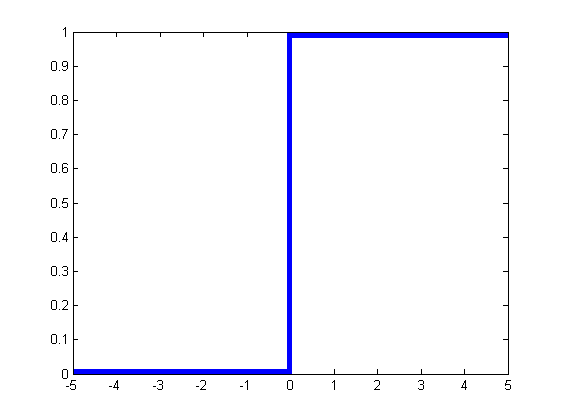
\includegraphics[width=.8\linewidth]{degrau}
	\caption{}
	\label{fig:ativacao:sub:degrau}
	\centering
\end{subfigure}\
\begin{subfigure}{.9\textwidth}
  \centering
  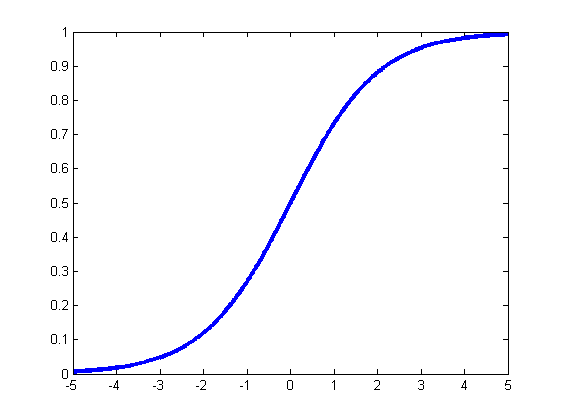
\includegraphics[width=.8\linewidth]{logistica}
	\caption{}
	\label{fig:ativacao:sub:logistica}
	\centering
\end{subfigure}
\caption{(a) Gráfico da função degrau com limiar 0. (b) Gráfico da função logística com a = 1}
\label{fig:ativacao}
\centering
\end{figure}

Outra função de interesse no estudo das redes neurais artificiais, é a função \textit{softmax} ou exponencial normalizada \cite{bishop2006pattern}. Essa função é utilizada na teoria estatística para a determinação da distribuição da probabilidade. Isto é, a função \textit{softmax} é uma função que define a probabilidade que uma varíavel discreta assuma um determinado valor\cite{altmanbs}. Em termos simples, o seu papel é transformar um vetor de $n$ elementos em um segundo vetor de mesmo tamanho, de valores no intervalo $[0,1]$ e que têm soma total igual a $1$.

Essa função é muito utilizada como função de ativação nas camadas de saídas de redes treinadas para reconhecimento de padrões, por sua capacidade de determinar a probabilidade da entrada pertencer a uma determinada classe. A função \textit{softmax} pode ser definida pela Equação \ref{eq:softmax}, onde $x$ é o vetor de tamanho $n$ da entrada e $x_i$ é o seu \textit{i-ésimo} elemento.

\begin{equation}
p(x)_i = \frac{\exp{x_i}}{\sum_{j=1}^n\exp{x_j}}
\label{eq:softmax}
\end{equation}




\section{Redes Neurais Feed-Forward}

Apesar de neurônios serem capazes de resolver alguns problemas sozinhos, o verdadeiro poder das redes neurais vem da interconexão entre os neurônios de forma a criar ligações semelhantes às sinapses dos neurônios naturais.

Existem várias arquiteturas para a formação destas redes de neurônios, porém neste trabalho a discussão será limitada àquela utilizada na implementação do programa: as chamadas redes neurais \textit{feed-forward}.

São necessárias ao menos três camadas para a construção da rede neste modelo: a primeira camada, chamada de camada de entrada, uma ou mais camadas intermediárias(ou ocultas) e a camada de saída. O papel das camadas ocultas é intermediar entre as entradas externas e a saída da rede, de forma a possibilitar que a rede extraia dados estatíticos mais significativos da sua entrada.  Uma camada é composta de um número de neurônios que agem de forma paralela. Cada neurônio de uma camada que não é a de saída está conectado a todos os neurônios da camada seguinte, de forma que não há comunicação entre uma camada e camadas anteriores a ela. Isto é, a informação flui na rede apenas no sentido entrada-saída, como ilustrado na Figura \ref{fig:feedfoward}.

\begin{figure}
\centering
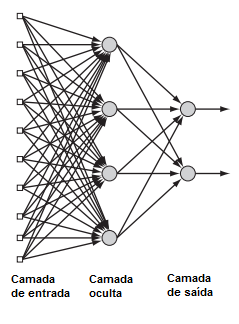
\includegraphics[width=.6\textwidth]{feedforward}
\caption{A arquitetura feed-forward. Cada neurônio se comunica com os neurônios da camada seguinte até que a saída final seja produzida. Adaptada de \cite{Haykin}.}
\label{fig:feedfoward}
\centering
\end{figure}

O vetor de entrada da rede é alimentado aos neurônios da primeira camada, cuja saída serve de entrada para a segunda camada e assim por diante, até que a última camada seja alimentada pela saída da camada anterior e produza a saída final da rede. 

\section{Treinamento}

Para que uma rede neural artificical possa ser utilizada, ela precisa antes aprender a realizar a tarefa para a qual foi criada. Para isso a rede precisa ter duas habilidades importantes: de aprendizado e de generalização. Aprendizado é a capacidade da rede de aproximar o comportamento das entradas fornecidas durante o treinamento, enquanto generalização é a sua capacidade de prever e operar sobre dados além do conjunto com a qual foi treinada\cite{ZhangNNSurvey}.

É necessário então que a rede passe por um processo de treinamento, onde os valores dos pesos $wi$ e os deslocamentos $b$ de cada neurônio são definidos de forma que o funcionamento da rede seja ótimo para a tarefa que se deseja realizar. Para realizar o treinamento de uma rede, o primeiro passo é definir 3 conjuntos distintos de entradas:

\begin{itemize}
	\item \textbf{Conjunto de treinamento:} A rede é submetida às entradas deste conjunto para que seja feita a calibração dos valores da matriz de pesos $W$ e do vetor de deslocamentos $B$.
	
	\item \textbf{Conjunto de validação:} Após uma etapa de treinamento, a rede computa os dados deste conjunto de entradas para validar os valores da matriz $W$ e do vetor $B$ escolhidos até então.
	
	\item \textbf{Conjunto de testes:} Por fim, após o treinamento, a rede é submetida aos dados deste conjunto, a fim de verificar o seu funcionamento correto.
\end{itemize}

Isto é, a cada ciclo de treinamento, a rede ajusta os seus pesos e deslocamentos de acordo com o conjunto de treinamento, e em seguida processa os dados do conjunto de validação. Se for determinado que a rede teve sucesso no processo de validação, ela fica pronta pra passar pelo conjunto de testes, aonde a sua capacidade de generalização é testada. A matriz $W$ de pesos gerada durante este processo é uma forma de representação do "conhecimento" da rede. Assim, o aprendizado não é uma característica de cada neurônio, mas sim um processo que ocorre na rede inteira como resultado do treinamento\cite{Kosabov}.

Existem duas principais maneiras de se executar o treinamento de uma rede.

\begin{itemize}
	\item \textbf{Treinamento supervisionado:} Neste paradigma os conjunto de treinamento e de validação consistem em um grupo de vetores de entrada $x$ e um gabarito de vetores de saída desejado $y$. O treinamento acontece até que o vetor de saída da rede para uma determinada entrada $x_i$ seja suficientemente próximo do vetor gabarito $y_i$ correspondete.
	
	
	\item \textbf{Treinamento não-supervisionado:} Neste paradigma a rede apenas recebe um conjunto $x$ de entradas e aprende características intrínsicas do dados apresentados a ela.
	
\end{itemize}

Uma vez definido o paradigma de treinamento, é necessário definir uma técnica para a análise do erro e alteração dos valores da matriz de pesos $W$ e do vetor $B$ de deslocamentos. Uma das técnicas mais utilizadas é a chamada de \textit{backpropagation}\cite{DeepLearning, ZhangNNSurvey}. A técnica consiste de uma análise do erro apresentado na saída da rede, que então é utilizada para se percorrer a rede no sentido contrário dos dados modificando os valores de $W$ e $B$ de forma a diminuir o erro na próxima iteração. Essa técnica é muito utilizada para sistemas de treinamento supervisionado, onde o erro é avaliado através de uma comparação da saída da rede com o gabarito fornecido. Uma vez que os valores de $W$ e $B$ param de mudar, diz-se que a rede atingiu um estado de convergência \cite{Kosabov} e o treinamento finaliza.


\section{Classificação de padrões}




Um problema muito comum que pode ser solucionado com redes neurais artificiais é o da classificação de padrões. Isto é, analisar um padrão ou um conjunto de características de um conjunto de dados e designá-lo a uma de várias classes pré-determinadas. Os nossos sentidos são muitas vezes capazes de fazer isso com extrema facilidade em uma fração de segundo. Por exemplo, se estamos andando pela rua, somos capazes de dizer que um som mais agudo e melódico é o canto de um pássaro, enquanto um som mais grave e contínuo provavelmente pertence ao motor de um carro passando. Essa habilidade é adquirida através de um aprendizado que ocorre durante as nossas vidas, e da mesma forma podemos ensinar uma rede neural artificial a reconhecer e classificar padrões.

Normalmente, uma rede que será utilizada para classificar padrões passa por um treinamento supervisionado, onde ela é alimentada com um vetor de entradas que contém características, ou \textit{features}, que descrevem os padrões junto com um gabarito que determina a classe a qual cada entrada pertence. Espera-se que depois do treinamento, ao ser apresentada a um novo padrão, a rede seja capaz de determinar a qual classe esse padrão pertence. Para que a rede demonstre boa generalização, é importante que ela não aprenda uma representação exata do conjunto de treinamento, mas que ela construa um modelo estatístico do processo que gera os dados \cite{NNForPR}.

\begin{figure}[!ht]
\centering
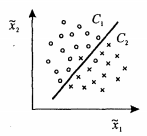
\includegraphics[width=5cm]{features}
\caption{Um gráfico que mostra duas características $\tilde{x}_1$ e $\tilde{x}_2$ de um problema de classificação hipotético. Círculos são padrões da classe $C_1$, enquanto os 'x' são padrões da classe $C_2$. O limiar de decisão, representado pela linha, consegue separar bem as duas classes quando as características são consideradas como um par. Porém haveria grande sobreposição se os valores fossem considerados separadamente. Extraída de \cite{NNForPR}.}
\label{fig:features}
\centering
\end{figure}

A escolha das características a serem utilizados para descrever os padrões não pode ser aleatória. Deve se escolher um número de características suficiente para descrever todos os padrões que podem ser encontrados. Além disso é importante que as características sejam suficientemente discriminantes. Isto é, deve haver o mínimo possível de superposição entre as características de classes distintas. Essas características podem ser escolhidos a mão, com base em um conhecimento prévio dos dados a serem classificados, ou extraídos automaticamente por um algoritmo desenvolvido para tal. Normalmente as características são processadas em conjunto e não consideradas individualmente. A Figura \ref{fig:features} mostra como isso é benéfico. Se as características hipotéticas $\tilde{x}_1$ e $\tilde{x}_2$ forem consideradas separadamente, há significativa superposição, de forma que é difícil separar com convicção as duas classes $C_1$ e $C_2$, porém, quando consideradas juntas, é possível traçar uma linha que as separa facilmente, apesar de alguns poucos elementos se confundirem. O papel da rede é determinar a função que traça essa linha através do treinamento, e retornar uma probabilidade de que um conjunto de características que lhe foi fornecido faça parte de uma determinada classe.



Um exemplo: se queremos criar uma rede que diferencia imagens de peixes palhaço de imagens de tubarões, um conjunto adequado de características provavelmente envolveria a cor $c$ predominante do animal, o tamanho do animal $t$ e o tamanho $b$ das suas barbatanas. A rede então seria submetida a entradas na forma de um vetor $(c, t, b)^T$, valores numéricos que caracterizam uma imagem a ser analisada. Podemos facilmente separar as classe através dessas características. Peixes com cor mais próxima do laranja e barbatanas pequenas são muito provavelmente peixes palhaços, enquanto aqueles que têm a barbatana grande seriam classificados como tubarões.